\documentclass[conference]{IEEEtran}

% Fix to revert the changes IEEEtran makes to table caption styles
\usepackage{etoolbox}
\makeatletter
\patchcmd{\@makecaption}
  {\scshape}
  {}
  {}
  {}
\makeatother
\usepackage[font=scriptsize,justification=justified,singlelinecheck=false]{caption}

%===========================================================================
\usepackage{listings}
\lstloadlanguages{C++}

% Settings for the lstlistings environment
\lstset{
language=C++,                       % choose the language of the code
basicstyle=\footnotesize\ttfamily,  % the size of the fonts that are used for the
                                    % code
numbers=none,                       % where to put the line-numbers
numberstyle=\tiny,                  % the size of the fonts that are used for the
                                    % line-numbers
stepnumber=1,                       % the step between two line-numbers. If it's
                                    % 1 each line will be numbered
numbersep=5pt,                      % how far the line-numbers are from the code
%backgroundcolor=\color{gray},      % choose the background color. You must add
                                    % \usepackage{color}
showspaces=false,                   % show spaces adding particular underscores
showstringspaces=false,             % underline spaces within strings
showtabs=false,                     % show tabs within strings adding particular
                                    % underscores
keywordstyle=\bfseries\color{blue},  % color of the keywords
commentstyle=\color{darkgreen},     % color of the comments
stringstyle=\color{darkred},        % color of strings
captionpos=b,                       % sets the caption-position to top
tabsize=2,                          % sets default tabsize to 2 spaces
frame=tb,                           % adds a frame around the code
breaklines=true,                    % sets automatic line breaking
breakatwhitespace=false,            % sets if automatic breaks should only happen
                                    % at whitespace
escapechar=\%,                      % toggles between regular LaTeX and listing
belowskip=0.3cm,                    % vspace after listing
morecomment=[s][\bfseries\color{blue}]{struct}{\ },
morecomment=[s][\bfseries\color{blue}]{class}{\ },
morecomment=[s][\bfseries\color{blue}]{public:}{\ },
morecomment=[s][\bfseries\color{blue}]{public}{\ },
morecomment=[s][\bfseries\color{blue}]{protected:}{\ },
morecomment=[s][\bfseries\color{blue}]{private:}{\ },
morecomment=[s][\bfseries\color{black}]{operator+}{\ },
xleftmargin=0.1cm,
%xrightmargin=0.1cm,
}

\usepackage{color}
\usepackage{comment}
\usepackage{graphicx}
\usepackage{amsmath}
\usepackage{amsfonts}
\usepackage[hidelinks]{hyperref}
\usepackage{cite}

\usepackage{fixme}
\fxusetheme{color}
\fxsetup{
    status=draft,
    author=,
    layout=inline, % also try footnote or pdfnote
    theme=color
}

%===========================================================================
\begin{document}
\title{Solving Large Quantities of Small Matrix Problems on Cache-Coherent SIMD Architectures}

%===========================================================================
% author names and affiliations
% use a multiple column layout for up to three different
% affiliations
\author{
\IEEEauthorblockN{Bryce Adelstein Lelbach, Hans Johansen, and Samuel Williams}
\IEEEauthorblockA{Computational Research Division, Lawrence Berkeley National Laboratory, Berkeley, CA 94720\\ {\it \{balelbach, hjohansen, swwilliams\}@lbl.gov}}
%\and
%\IEEEauthorblockN{Homer Simpson}
%\IEEEauthorblockA{Twentieth Century Fox\\
%Springfield, USA\\
%Email: homer@thesimpsons.com}
}

% conference papers do not typically use \thanks and this command
% is locked out in conference mode. If really needed, such as for
% the acknowledgment of grants, issue a \IEEEoverridecommandlockouts
% after \documentclass

% for over three affiliations, or if they all won't fit within the width
% of the page, use this alternative format:
% 
%\author{\IEEEauthorblockN{Michael Shell\IEEEauthorrefmark{1},
%Homer Simpson\IEEEauthorrefmark{2},
%James Kirk\IEEEauthorrefmark{3}, 
%Montgomery Scott\IEEEauthorrefmark{3} and
%Eldon Tyrell\IEEEauthorrefmark{4}}
%\IEEEauthorblockA{\IEEEauthorrefmark{1}School of Electrical and Computer Engineering\\
%Georgia Institute of Technology,
%Atlanta, Georgia 30332--0250\\ Email: see http://www.michaelshell.org/contact.html}
%\IEEEauthorblockA{\IEEEauthorrefmark{2}Twentieth Century Fox, Springfield, USA\\
%Email: homer@thesimpsons.com}
%\IEEEauthorblockA{\IEEEauthorrefmark{3}Starfleet Academy, San Francisco, California 96678-2391\\
%Telephone: (800) 555--1212, Fax: (888) 555--1212}
%\IEEEauthorblockA{\IEEEauthorrefmark{4}Tyrell Inc., 123 Replicant Street, Los Angeles, California 90210--4321}}




% use for special paper notices
%\IEEEspecialpapernotice{(Invited Paper)}




% make the title area
\maketitle

%===========================================================================
\begin{abstract}
A number of computational science algorithms lead to discretizations
  that require a large number of independent, small matrix solves.
Examples include small non-linear coupled chemistry and flow systems,
  one-dimensional sub-systems in climate and diffusion simulations, 
  alternating direction implicit pre-conditioners, and 
  semi-implicit time integrators, among others.
We present a performant approach for solving large quantities of 
  independent matrix problems on cache-coherent SIMD architectures. 
Unlike many vectorized or ``batched'' approaches that rely on reusing
  the matrix factorization across multiple solves, our algorithm supports
  the case of sets of matrices that are different, due to
  spatial variation or non-linear solvers, for example.
We demonstrate the approach with a prototypical tridiagonal matrix solver,
  derived from a 1D solver that is part of an implicit-explicit 
  finite difference discretization for a 3D advection-diffusion problem.
Performance is evaluated on several Intel architectures with different cache,
  vectorization, and threading features, and compared to theoretical
  roofline models across parameter studies.
We conclude that the approach is effective at optimizing both vectorization 
  and memory bandwidth, and improves on existing approaches for efficiently
  solving large numbers of small matrix problems.
\end{abstract}

% no keywords


% For peer review papers, you can put extra information on the cover
% page as needed:
% \ifCLASSOPTIONpeerreview
% \begin{center} \bfseries EDICS Category: 3-BBND \end{center}
% \fi
%
% For peerreview papers, this IEEEtran command inserts a page break and
% creates the second title. It will be ignored for other modes.
\IEEEpeerreviewmaketitle

%===========================================================================
\section{Introduction}
% 
One important class of problems in computational science is the solving
  of smaller-dimensional matrix subproblems that are duplicated across
  many degrees of freedom in a larger two or more dimension computation.
Several examples of this include: 
\begin{itemize}
\item Pointwise chemistry systems in the context of a larger, 
  flow simulations. 
Examples include geochemistry~\cite{??}, cloud microphysics~\cite{??},
  and combustion~\cite{??};
\item Solving one-dimensional systems that represent a ``primary''
  direction for a physical phenomenon.
Examples here include atmospheric radiation~\cite{??}, groundwater
  penetration~\cite{??}, or models for cloud convection~\cite{??}; and
\item Implicit solvers that need to couple these kinds of subsystems, 
  such as physics-based preconditioners~\cite{??}, alternating 
  direction implicit ADI,~\cite{??}, and operator-split or
  semi-implicit time integrators~\cite{??}.
\end{itemize}
In most cases, these matrices are relatively small 
  (ranging from $O(10-100)$ chemistry components or ``levels'' 
  in a climate application), and may be sparse or dense, but must 
  be solved repeatedly, but with different entries each time, 
  to advance the overall simulation.
Thus, because these are often non-linear matrix systems with space- and 
  time-dependent entries, these applications may not use a 
  ``factor once, solve many times'' approach, which is often used 
  as a model matrix performance test.
This prevents amortizing setup and factorization costs
  across multiple right-hand side solves as in \emph{dgxxxxx}~\cite{??},
  and also challenges SIMD vectorization due to the odd size and
  dissimilar entries of the matrices, as well as the 
  memory access patterns relative to the bigger simulation data layout.
In that case, it is usually sub-optimal on many-core SIMD 
  or SIMT GPU architectures
  to simply call an optimized linear algebra library, 
  such as Intel's MKL version of LAPACK~\cite{mkl_website} or NVIDIA's
  cuBLAS~\cite{cublas_website}; these may not achieve peak memory bandwidth 
  and VPU performance across the range of small matrix size. 
In that sense, it can leads applications to create their own 
  custom implementations, which may not be optimal, and create a 
  (potentially unnecessary) maintenance burden for the applications 
  running across multiple many-core architectures as well. 
  
To this end, we have developed a model matrix kernel that mimics what
  is encountered in these kinds of large-scale simulations.
Key aspects of the code include:
\begin{itemize}
\item Matrix systems that must be created and solved
  at each point in a two-dimensional subdomain (represented by $(i,j)$ indices)
  of a three-dimensional application (that is, $(i,j,k)$ indices).
\item Each matrix is tri-diagonal, and must be solved for all $O(30-100)$
  values in the $k$ index.
\item The matrix is derived from finite difference discretization for the
  1D diffusion equation, which allows it to be solved without pivoting
  (pivoting will be addressed in future work).
\end{itemize}

%===========================================================================
\section{Related Work}
Approaches to solving large numbers of small matrices have been done
  in a variety of contexts.
Many implementations simply solve each matrix in parallel or for multiple
  right-hand sides, using platform-specific
  implementations of LAPACK, such as Intel's Math Kernel Library~\cite{mkl_website}
  or NVIDIA's cuBLAS~\cite{cublas_website} implementations.
In many cases, there is a benefit from vectorization and thread parallelism, 
  but there may be overheads that reduce performance such as data copies
  into local arrays, dynamic determination of optimal performance parameters, 
  partially vectorized ``peel'' loops, etc.~\cite{??}.
Some specialized approaches include specialized linear algebra-specific 
  compilers for small problem sizes and target architectures 
 ~\cite{Spampinato:2014, ??} \fxnote{(add build-to-order ref, Siek/Jessup?)}.
Other libraries like 
  \emph{Blaze}~\cite{BlazeSite}, 
  \emph{PLASMA}~\cite{PLASMASite},
  \emph{MAGMA}~\cite{Haidar:2015}, and 
  \emph{libxsmm}~\cite{libxsmm_website}
  are intended to support SIMD vectorization for standard vector sizes
  as well as batched computation for sparse and dense matrices.
Overall, there is a gap in approaches that both have vectorization,
  regardless of matrix size, with or without dense/sparse/pivoting 
  assumptions, amortizing factorization across multiple right-hand-sides, 
  and other assumptions.
\\
\fxnote{(Hans - fill in more background / details on these.)}

%===========================================================================
\section{Implementation}

Suppose we have a symmetric positive-definite or diagonally-dominant $n$x$n$
tridiagonal matrix $A$ and two $n$-element vectors $u^{s}$ and $u^{s+1}$. We
wish to solve $Au^{s+1} = u^{s}$ for $u^{s}$:

\[
\begin{bmatrix}
b_0 & c_0 &     &         & 0       \\
a_1 & b_1 & c_1 &         &         \\
    & a_2 & b_2 & ...     &         \\
    &     & ... & ...     & c_{n-2} \\
0   &     &     & a_{n-1} & b_{n-1}
\end{bmatrix}
\begin{bmatrix}
u^{s+1}_0     \\
u^{s+1}_1     \\
...     \\
...     \\
u^{s+1}_{n-1}
\end{bmatrix}
=
\begin{bmatrix}
u^{s}_0     \\
u^{s}_1     \\
...     \\
...     \\
u^{s}_{n-1}
\end{bmatrix}
\]

Our matrix $A$ is stored as a set of three vectors: an $n-1$-element
sub-diagonal vector $a$, an $n$-element diagonal vector $b$ and an $n-1$-element
super-diagonal vector $c$.

We can use a simplified form of Gaussian elimination which does not perform any
pivoting to solve such a system. This method is known as the Thomas algorithm
or the tridiagonal matrix algorithm (TDMA)~\cite{TDMA}, and it is \(O(n)\) in time,
a significant improvement over full Gaussian elimination for a completely dense
matrix, which is \(O(n^3)\) in time. We use the in-place Thomas algorithm,
which does not require any storage for temporary values but overwrites the $b$
vector. We will also solve for $u^{s+1}$ in-place, overwriting $u^{s}$ (so our
system is $Au$).

% Citation here is elementary numerical analysis
The in-place Thomas algorithm consists of two passes. First, a forward pass is
performed to eliminate the $a_i$ elements~\cite{??}:

\begin{lstlisting}
for (auto k = 1; k < n; ++k) {
  auto const m = a[k] / b[k - 1];
  b[k] = b[k] - m * c[k - 1];
  u[k] = u[k] - m * u[k - 1];
} 
\end{lstlisting}

Then, an abbreviated form of backwards substitution is performed to obtain the
solution~\cite{??}:

\begin{lstlisting}
u[n - 1] = u[n - 1] / b[n - 1];

for (auto k = n - 2 ; k >= 0; --k) {
  u[k] = (u[k] - c[k] * u[k + 1]) / b[k];
} 
\end{lstlisting}

\fxnote{Paragraph describing AI}

\subsection{Division Optimizations}

% 1st Reference here is Intel Optimization Manual, 11.12
% 2nd Reference here is the intrinsic manual
When we analyzed implementations of the Thomas algorithm as described above, we
observed that while the it is primary memory-limited, performance could be
sensitive to the latency of the floating point divisons present in the
algorithm. Vectorized floating point operations which use the division
execution unit (divides, fast reciprocal estimation, square root) are not
pipelined on many mainstream architectures, including Intel SSE, AVX and AVX2
platforms~\cite{}. Thus, these operations have very high latency (43 cycles for
an AVX 256-bit double-precision divide on Sandy Bridge; 35 cycles on Ivy Bridge
and Haswell~\cite{}) and low throughput relative to other floating point
operations such as multiplication and addition.

In the in-place Thomas algorithm described above, all the division operations
have the same divisor - the temporary coefficient computed and stored in the
diagonal vector \(b\). If we re-formulate the algorithm to store the reciprocal
of that coefficient instead of storing the coefficient itself, we are able to
remove the division in the backwards substitution pass. We call this the
\textbf{cached-divide} in-place Thomas algorithm. The forward elimination pass
is:

\begin{lstlisting}
b[0] = 1.0 / b[0];

for (auto k = 1; k < n; ++k) {
  auto const m = a[k] * b[k - 1];
  b[k] = 1.0 / (b[k] - m * c[k - 1]);
  u[k] = u[k] - m * u[k - 1];
} 
\end{lstlisting}

The backwards substitution pass becomes:

\begin{lstlisting}
for (auto k = n - 2 ; k >= 0; --k) {
  u[k] = (u[k] - c[k] * u[k + 1]) * b[k];
} 
\end{lstlisting}

\fxnote{Paragraph discussing the changes in AI with cached variant}

\fxnote{Revive the RCPPS optimization section}

%One well-known technique for optimizing floating point divisions is to replace
%division operations with fast reciprocal estimates (RCP) when possible. On many
%platforms where floating point division operations are not pipelined, floating
%point RCP operations will also not be pipelined, however they generally have
%much lower latency and higher throughput than division operations. Many
%optimizing compilers will transparently and reliable perform this optimization.
%However, there is a caveat on 256-bit AVX and AVX2 platforms (e.g. Sandybridge,
%Ivy Bridge, Haswell and Skylake); no double-precision RCP is available on these
%platforms, although a single-precision RCP instruction is available.
%
%% TODO: Probably give this a name.
%
%We experimented with the use of a single-precision RCP and Newton Raphson
%iteration to compute a fast division estimation. We are not aware of a compiler
%which provides optionally provides this optimization. To implement the
%optimization, we simply type cast the double-precision values to
%single-precision, perform a division operation, cast back to double-precision
%and then preform Newton Raphson iterations (at double precision). We rely on
%the compiler to replace the division with an RCP instruction.
%
%\begin{lstlisting}
%template <std::size_t NRIterations = 1>
%double nr_rcp_divide(double num, double den) {
%  double x = float(1.0) / float(den);
%
%  for (auto i = 0; i < NRIterations; ++i)
%    x = x + x * (1.0 - den * x);
%
%  return num * x;
%}
%\end{lstlisting}
%
%Since the single-precision RCP instruction will operate on twice as many values
%as a double-precision division from the same instruction set, when our division
%estimate is used in a vectorized loop it is prudent to unroll the loop at least
%once so that one single-precision RCP instruction can service two
%double-precision iterations. Again, we have been able to rely on the compiler
%to handle this component of the optimization.
%
%We do pay an overhead for the type conversion, in the form of packed-double to
%packed-single vector instructions. Additional double-precision multplications
%and additions are also needed, even with 0 Newton Raphson iterations.
%Section~\ref{} and Table~\ref{} discuss the performance of this division
%estimate and the tradeoff in accuracy.
%
%\fxnote{Paragraph explaining why we're not actually doing this.}

% Maybe call this Algorithmic Strategy?
\subsection{Batching Strategy}

In the applications described in Section~\ref{??}, we need to compute the
solution to a tridiagonal system via the Thomas algorithm on each vertical
(e.g. $z$) column in a $nx \times ny \times nz$ Cartesian grid (Figure~\ref{1}).
These computations are known as the \textbf{vertical solves}. The matrix
coefficients for each column depend on the problem state, so a unique matrix
for each column needs to be constructed before each solve. There are two
different approaches to computing these batch solves: solve each column
independently, or simultaneously solve multiple columns.

The most straightforward approach is to deal with each tridiagonal solve
separately, independent of the other solves. An $nz\times nz$ tridiagonal
matrix is constructed for each column, and then the Thomas algorithm is used to
solve the system formed by the matrix and the vertical column. Because the
column solves are independent, different column solves can be executed
concurrently via task-level parallelism. Vectorization of the $nz$ loop is
not possible as each iteration of the solve is dependent on previous iterations.

The other approach is to simultaneously solve multiple columns. A block
$nz \times nz$ tridiagonal matrix is constructed for the whole grid; each block
contained within the matrix is an $nx \times ny$ horizontal plane (e.g. the
block matrix is a 4D space). The entire 3D Cartesian grid is viewed as an
$nz$ block vector of $nx \times ny$ planes. The Thomas algorithm is then
applied to the block matrix; each step of the algorithm is applied across an
entire plane. For example, the forward sweep becomes:

\begin{lstlisting}
for (auto j = 0; j < ny; ++j)
  for (auto i = 0; i < nx; ++i) 
    b[i][j][0] = 1.0 / b[i][j][0];

for (auto k = 1; k < nz; ++k)
  for (auto j = 0; j < ny; ++j)
    for (auto i = 0; i < nx; ++i) {
      auto const m = a[i][j][k] * b[i][j][k - 1];
      b[i][j][k] = 1.0 / (b[i][j][k] - m * c[i][j][k - 1]);
      u[i][j][k] = u[i][j][k] - m * u[i][j][k - 1];
    } 
\end{lstlisting}

This approach facilities both task-level parallelism and vectorization. The
grid and block matrix can be tiled into smaller subgrids, and the Thomas
algorithm can be applied to each subgrid independently. Each step of the Thomas
algorithm can be vectorized across the $nx \times ny$ horizontal plane that it
is operating on: e.g. the j or i loops in the above snippet can be vectorized.
The innermost loop can be vectorized, the innermost loop can be unrolled and
the next-innermost loop can be vectorized, or the two innermost loops can be
collapsed and vectorized.

\fxnote{TODO: Explain that the independent solve approach is what LAPACK does,
and that's why it is insufficient for this type of problem. Also, explain that
LAPACK has no routine for Thomas-style tridiagonal solves - dgtsv is
generalized, does actual Gaussian eliminiation and may do pivoting. Also
mention somewhere that MKL does not parallelize dgtsv.}

The vector parallelism exposed by the simultaneous approach offers a major
benefit over the independent approach, since it is not possible to vectorize
most of the kernels in the independent approach due to data dependencies
between iterations of the Thomas algorithm. Even if it was possible to
vectorize in the vertical $nz$ dimension, it would still be undesirable to do
so. The extent of the vertical dimension tends to be very small in the
applications we are concerned with\fxnote{HOW SMALL}. Vectorizing in the
horizontal dimensions allows us to control locality and loop trip counts via
tiling.

\subsection{Data Layout}

The data layout of the Cartesian grid has a huge impact on the performance
potential of the vertical solves. Throughout the course of our research, our
understanding of the impact of different data layouts has evolved
substantially. We have investigated three different schemes:

% kji AKA column-major, Fortran, left
% ijk AKA row-major, C++, right
\begin{tabular}[t]{c|c|c|c} \hline
\textbf{Name}         & \textbf{i-stride} & \textbf{j-stride} & \textbf{k-stride}   \\
                      &                   &                   & \textbf{(Vertical)} \\ \hline
\(ijk\), Column-Major & \(1\)             & \(nx\)            & \(nx * ny\)         \\ 
\(kji\), Row-Major    & \(ny * nz\)       & \(nz\)            & \(1\)               \\ 
\(ikj\)               & \(1\)             & \(nx * nz\)       & \(nx\)              
\end{tabular}

The production codebase we are analyzing currently uses the \(ijk\) layout. The
codebase is based on the Chombo C++ framework, which typically uses this layout
(column-major) for interoperability with Fortran kernels. The vertical solves
in this codebase are calculated using LAPACK. In this layout, the vertical
dimension (\(k\)) has the greatest stride. Thus, the vertical column that we
need to pass in to LAPACK as the solution vector (\(u\)) will be non-contiguous
and will have little to no innate locality between elements. Currently, the
production codebase allocates a temporary buffer, copies data from the grid
into the buffer, calls the LAPACK solver, and then copies the result from the
temporary buffer back to the grid.

Initially, we investigated switching to the \(kji\) layout, which would give us
contiguous vertical columns that could be passed into LAPACK and allow us to
remove these temporary buffer allocations. We observed a noticeable performance
increase from this change with very little source code impact (the production
codebase we are working with does not need to interoperate with Fortran). We
have not studied the impact of this layout change on the explicit horizontal
stencil in detail.

% TODO: You've got to reference a section where you explain why it's not sufficient
Eventually, we determined that LAPACK would not be sufficient for the vertical
solves and that we could achieve substantially higher bandwidths by developing
the solver described in this paper, we revisited the data layout question. As
we would not be able to vectorize the Thomas algorithm in the vertical
dimension due to the the loop-carried dependencies present in the algorithm, we
decided to switch back to an \(ijk\) layout, where one horizontal dimension (\(i\))
is the unit stride dimension and the vertical dimension (\(k\)) has the greatest
stride.

The next layout we investigated, the \(ikj\) layout, arose as a solution to
translation lookaside buffer (TLB) performance issues that we encountered after
developing and studying a tiling abstraction for our solver. It is described in
greater detail in the next section.

\subsection{Tiling}

\fxnote{Elaborate on distinction between entire tile/per array tile.}

To ensure good CPU cache utilization, it is often necessary to break a larger
grid into smaller tiles which have greater data locality and can fit into a
particular CPU cache. The Thomas algorithm is no exception. In particular, we
want all four arrays (\(a\), \(b\), \(c\) and \(u\)) to remain in cache in
between the forward elimination and the back substitution loops. Our analytical
performance model is based on this assumption. If any of these four arrays need
to be reloaded from main memory in between the forward elimination and back
substitution loops, the amount of main memory data movement is significantly
increased and the algorithmic intensity of the algorithm decreases notably. Of
course, tiling also provides a useful abstraction for parallelization, as each
tile can be computed independent of any other tiles and has no overlapping data
accesses.

The original production code which we worked with did not do any tiling. Since
each column was solved by a LAPACK call, completely independent of any other
columns, the improved data locality exposed by tiling could not be fully
exploited. In the original \(ijk\) layout production code, a contiguous buffer
was created to gather the non-contiguous column from the 3D grid, and the
matrix was built on the fly for each column. Our NAMEFORALGO was designed from
the ground up to both simultaneously build the matrix and simultaneously solve
multiple columns. It was evident that we would need to add a tiling abstraction
to our implementation. While our un-tiled results beat the reference MKL
results (see Figure \ref{}), they were well below the manufacturer-specified
bandwidth and profiling made it clear that cache performance was the culprit.

Due to the loop-carried dependencies in the Thomas algorithm, we could not tile
the vertical dimension. Even if we could, this would be undesirable because the
vertical dimension is typically quite small \fxnote{HOW SMALL}. Thus, our tiling 
abstraction would need to subdivide the horizontal \(ij\) plane.

Our initial implementation used an \(ijk\) layout, where one of the horizontal
dimensions (\(i\)) is the unit stride dimension, the other horizontal dimension
(\(j\)) has the next smallest stride and the vertical dimension (\(k\)) has the
greatest stride.

We decided to only tile in one of the horizontal dimensions (\(j\), the
non-unit stride horizontal dimension), to minimize the number of non-contiguous
memory regions in each tile. Consider two different tiling regimes: the "tile
both" approach subdivides both the \(i\) and \(j\) dimensions by \(x/2\), and
the "tile \(j\)" approach subdivides only the \(j\) dimension by \(x/4\) (we
assume here that \(y\) is divisible by \(x/2\) and thus can be neatly tiled in
this manner). Both approaches create tiles of containing the same number of
elements, and conceptually will fit into the same space in a data cache
(\(x/2\)x\(x/2\)x\(z\) tiles for "tile both" and \(x\)x\(x/4\)x\(z\) tiles for
"tile \(j\)"). However, the "tile \(j\)" approach has much greater data
contiguity. For the "tile \(j\)" approach, we have \(z\) contiguous
\(ij\)-planes, each containing \(x\)x\(x/4\) elements.  For the "tile both"
approach, we have \((x/2)*z\) contiguous \(i\)-lines, each containing \(x/2\)
elements.

The greater contiguity of the "tile \(j\)" approach means fewer strided
accesses and more importantly fewer translation lookaside buffer (TLB) entries
needed per tile. In the worst case, assuming that each contiguous region of the
tile can fit within a single TLB entry and that a single entry cannot cover
multiple contiguous regions, the "tile both" case would take up \((x/2)*z\) TLB
entries, while the "tile \(j\)" approach would only need \(z\) TLB entries.

The only notable downside to the "tile \(j\)" approach versus the "tile both"
approach is the loss of flexibility in tile sizes. The smallest tile size for
the "tile \(j\)" approach is a \(x\)x\(1\)x\(z\) tile (a line of columns),
while the smallest tile size for the "tile both" approach is a
\(1\)x\(1\)x\(z\) tile (a single column). We do not believe this restriction is
problematic. Because we are vectorizing in the \(i\) direction, it is assumed
that the \(i\) dimension of a tile will be at least the size of the vector
width of the target platform. In practice, our vectorizing compiler typically
unrolls the loops in NAMEFORALGO after vectorization to amortize loop overheads
and fully utilize the vector register file. Thus, we typically use 2 or 4 times
the vector width as the minimum \(i\) dimension. 

We used the \(ijk\) layout and the "tile \(j\)" scheme for much of our initial
work. Part of our work was to study the effect of tile size on application
performance.  Tile size controls both the data locality and the parallel grain
size in our algorithm. Note that given the embarrassingly parallel nature of
this problem, the effect of tile size on parallelism is well known, and thus
are mostly outside of our consideration: tile sizes which are too small will
perform poorly due to high parallel overheads (the "left side" of the
traditional grain size parabola) and tile sizes which are too large will expose
insufficient parallelism leading to starvation (the "right side" of the
traditional grain size parabola)~\cite{some_parallex_thing}.

To determine an optimal tile size, we performed parameter sweeps of the domain
of tile sizes. We predicted four things:

\begin{itemize}
\item Tile sizes small enough to fit into the L1D cache would not be feasible
because the overheads of loop constructs, parallelization and vectorization
would be too great relative to the execution time of useful work per
inner-iteration ("left side" effect). These tile sizes would either require
smaller vertical dimensions than we use in the production application (\(k <
16\)) or horizontal dimensions too small to vectorize efficiently (\(i < 16\)).
\item The optimal tile size would fit into the L2 cache.
\item There would be a drop in performance for tile sizes which were too large to fit into the L2 cache.
\item There would be a drop in performance for tile sizes which were too large to fit into the L3 or HBM cache.
\item Sufficiently large tile sizes would express insufficient parallelism and
perform poorly due to starvation ("right side" effect).
\end{itemize}

Our predictions about tile sizes small enough to fit into the L1D cache held,
as did our predictions about sufficiently large tile sizes. Additionally, as we
expected, we saw a notable decrease in performance for tile sizes which were
too large to fit into the L3 cache (see Figure \ref{}), although on
microarchitectures with a shared L3 cache we did not see this effect in our
single core results (see Figure \ref{}). Our 

However we were intrigued to find that, across multiple microarchitectures, the
tile size which gave the best performance was often a tile size which did
\emph{not} fit into the L2 cache (see Figure \ref{}). The optimal tile size for
the \(ijk\) layout version of NAMEFORALGO was usually either equal to or
slightly larger than the size of the L2 (see Figure \ref{}). Note that if the
tile size is equal to the size of the cache, we would not consider it to be
small enough to fit in that cache, as we cannot reasonably expect perfect cache
utilization or that our four arrays (\(a\), \(b\), \(c\) and \(u\)) will be the
only data that needs to be stored in the cache. This result was surprising; we
had expected a notable drop in performance for these tiles sizes because the
arrays would need to be reloaded from the L3 cache (or the HBM cache in the
case of the KNL) at the start of each loop in the kernel. 

When profiling the code, we noticed poor TLB performance, and came to the
realization that this was the cause of the problem. As we discussed earlier, we
were using the "tile \(j\)" scheme with the \(ijk\) layout version of
NAMEFORALGO. This scheme offers better data contiguity than the alternate "tile
both" scheme, however, we still end up with a non-contiguous tile.  The number
of contiguous regions (and thus TLB entries) were quite large relative to
hardware capabilities. Even worse, for smaller tile sizes, the size of each
contiguous region accessed might be less than the smallest page size available
on the microarchitectures we investigated (4KB in all cases). This would mean
that for smaller tile sizes, we were not fully utilizing each TLB entry.  Our
strategy for aligning and padding our arrays to avoid data cache conflicts
(described in Section \ref{}), while effective, meant that it was almost
guranteed that no two contiguous regions would reside on the same 4KB or 2MB
page, amplifying the problem. We have not yet definitely determined whether
huge pages (1GB) are being used in our benchmark via transparent huge page
support~\cite{}, and, if not, whether huge pages would be to mitigate this
effect.

As an example of this issue, \fxnote{EXAMPLE FROM A FIGURE}.

We concluded that as we decreased tile size, this TLB effect increasingly
became the dominant driving performance factor. A problem size that fit into
the L3 cache but did not fit into the L2 cache would have better performance
than a problem size that fit into the L2 cache because the former would make
better use of TLB entries and exert less pressure on address translation
hardware.

We soon realized that the problem was that we had decided that the
vertical dimension \(k\) should have the greatest unit stride (e.g. \(ijk\)
layout). However, we could not tile in the \(k\) for the same reason that we
cannot vectorize in the \(k\) dimension; there are loop-carried dependencies in
the Thomas algorithm. Because we could not tile in \(k\) and \(k\) had the greatest
stride, there was no way to subdivide our problem into contiguous tiles.
Consider planar slices of a \(ijk\) layout grid. \(ij\) planes are contiguous
(but require slicing in \(k\), which we cannot do), \(ik\) planes ("tile \(j\)"
approach) are non-contiguous and \(jk\) planes are non-contiguous.

Once we realized that the \(ijk\) layout was restricting us to a non-optimal
tiling scheme, we revisited the question of data layout in NAMEFORALGO.
Originally, we had one requirement: one of the horizontal dimension should be
the unit stride dimension so that we can vectorize in that direction. Now, we
had a second requirement: the vertical dimension should not be have the
greatest unit stride, because we cannot tile in the vertical dimension.
Naturally, this led us to the \(ikj\) layout, where the horizontal dimension
\(i\) is the unit stride dimension, the vertical dimension \(k\) has the next
smallest stride and the horizontal dimension \(j\) has the greatest unit
stride. We still use a "tile \(j\)" scheme, however, now our tiles are one
contiguous region instead of a set of \(z\) planes.

\fxnote{Interesting decision between ikj iteration vs ijk iteration in the ikj layout. May want to talk about that.}

The change to the \(ikj\) layout produced the desire result. On Sandybridge,
Ivy Bridge and Haswell, we saw a notable improvement in performance for smaller
tile sizes (see Figure \ref{}). On these microarchitectures, the best result
from the \(ikj\) layout variant matched or beat best result of the \(ijk\)
layout using a smaller tile size which would fit into the L2 cache.
\fxnote{DESCRIBE RESULTS}. On Knight's Landing, the impact was substantially
larger (see Figure \ref{}). \fxnote{DESCRIBE RESULTS}. The difference in impact
between the Intel Xeon architectures and Knight's Landing can be explained by
the lack of a traditional L3 cache on the Knight's Landing. With the \(ijk\)
layout on the KNL, the larger tile sizes which did not fit into the L2 cache would
have to rely on the HBM cache. While the HBM on the KNL provides substantial
bandwidth, when the HBM is configured to act as a last-level cache it provides
higher latencies than the typical L3 cache on an Intel Xeon would. We believe
this difference in cache latency explains the poorer performance relative to
manufacturer-specified bandwidth of the \(ijk\) layout, and thus explains the
more significant impact of the \(ikj\) layout on the KNL.

\subsection{Mitigating Cache Conflicts}

In addition to to data layout selection and tiling, it was necessary for us to
mitigate potential data cache conflicts, to ensure optimal cache performance.
It is necessary to both align and pad the four arrays used in our solver to
avoid accessing array elements which have addresses that are structurally
similar enough to be mapped to the same cache set (e.g. two addresses which are
aligned to the same power of two).

The loops in our algorithm will always access elements of four different arrays
with the same horizontal (\(ij\)) indices, and will access at most two
different adjacent vertical (\(k\)) indices. So, to avoid conflicts we must ensure 
that:

\begin{itemize}
\item \textbf{Inter-Array Conflicts} Elements of different arrays which have the same \(ijk\) indices map to different cache sets.
\item \textbf{Vertical Conflict} Elements of the same array which share the same \(ij\) indices map to different cache sets.
\end{itemize}

As described in the previous section, we expected the optimal tile size for
NAMEFORALGO to be small enough to fit into the L2 cache, so our cache conflict
considerations only account for L1D and L2 cache conflict misses. Note the
formula for the size of a set-associative cache (brackets denote units):

\begin{table*}[t]
\centering
\caption{\textbf{Formulae for Cache Conflict Mitigation Parameters:}}

\begin{align*}
CacheSize \: \text{[Bytes]} = Associativity \: \text{[Ways]} * CacheLineSize \: \text{[Bytes]} * NumberOfSets \: \text{[Sets]}
\end{align*}

\begin{align*}
BytesPerWay \: \text{[Bytes / Way]} = CacheSize \: \text{[Bytes]} / Associativity \: \text{[Ways]}
\end{align*}

\begin{align*}
L1DArrayAlignStep \: \text{[Bytes]} &= L1DBytesPerWay \: \text{[Bytes / Way]} \: / \: 4 \: \text{[Arrays]} \\
L2ArrayAlignStep \: \text{[Bytes]}  &= L2BytesPerWay \: \text{[Bytes / Way]}  \: / \: 4 \: \text{[Arrays]} \\ 
ArrayAlignStep \: \text{[Bytes]}    &= L1DArrayAlignStep \: \text{[Bytes]} + L2ArrayAlignStep \: \text{[Bytes]}
\end{align*}

\begin{align*}
L1DPlanePadding \: \text{[Bytes]} &= L1DBytesPerWay \: \text{[Bytes / Way]} \: / \: nz \: \text{[\# of Vertical Levels]} \\ 
L2PlanePadding \: \text{[Bytes]}  &= L2BytesPerWay \: \text{[Bytes / Way]}  \: / \: nz \: \text{[\# of Vertical Levels]} \\
PlanePadding \: \text{[Bytes]}    &= L1DPlanePadding \: \text{[Bytes]} + L2PlanePadding \: \text{[Bytes]}
\end{align*}

\begin{align*}
LinePadding \: \text{[Bytes]} = L1DBytesPerWay \: \text{[Bytes / Way]} \: / \: nz \: \text{[\# of Vertical Levels]}
\end{align*}

\label{tab:conflict_mitigation_formulae}
\end{table*}

\begin{table*}[t]
\centering
\caption{\textbf{Example Cache Conflict Mitigation Parameters}}

\fxnote{KILL THIS}

\label{tab:example_conflict_mitigation_parameters}
\end{table*}

To deal conflicts between elements of different arrays with the same
\(ijk\) indices, we align the base of each array differently. Assuming that all
the arrays are the same size, this ensures that the elements with the same
\(ijk\) indices in all four arrays will also be aligned differently. While
arrays \(b\) and \(c\) technically have one fewer vertical levels than \(u\)
and \(a\), for simplicity we allocate an equal amount of storage for all four
arrays. Each array is aligned to \(ArrayBaseAlign+nA*ArrayAlignStep\)
where \(nA\) is \(0\) for \(u\), \(1\) for \(a\), \(2\) for \(b\) and \(3\) for
\(c\).

\(ArrayBaseAlign\) should be a power of 2; 1MB is used for all the results
presented in this paper. \(ArrayAlignStep\) is the sum of two values,
\(L1DArrayAlignStep\) and \(L2ArrayAlignStep\), which are computed based on the
properties of the L1D and L2 caches on the target microarchitecture. The formulae
are shown in Table \ref{tab:conflict_mitigation_formulae}. 

To address conflicts between elements of the same array which have the same
\(ij\) indices but reside on two separate, adjacent vertical levels, our
strategy depends on the layout used. For the \(ijk\) layout, we need to add
padding \(PlanePadding\) at the end of each contiguous horizontal (\(ij\))
plane to ensure that vertical neighbors are not structural similar (e.g.
aligned to the same power of 2). \(PlanePadding\) is added to the \(k\) stride,
e.g. the indexing formula changes from:

\[
i + nx * j + nx * ny * k
\]

\noindent to:

\[
i + nx * j + (nx * ny + PlanePadding) * k
\]

\noindent \(PlanePadding\) is calculated similar to \(ArrayAlignStep\) (Table \ref{tab:conflict_mitigation_formulae}).

We have found that the storage overhead of \(PlanePadding\) (shown below in
Table \ref{tab:example_conflict_mitigation_parameters}) is relatively small for
non-trivial problems. \fxnote{IS THIS TRUE?}

A similar approach could be used to deal with these vertical cache conflicts
when using the \(ikj\) layout. Instead of adding \(PlanePadding\), we would add
\(LinePadding\) at the end of each contiguous \(i\) line. The indexing formula
would change from:

\[
i + nx * nz * j + nx * k
\]

to:

\[
i + (nx + LinePadding) * nz * j + (nx + LinePadding) * k
\]

In the \(ikj\) layout, the tile for each array is a contiguous region which is
small enough to fit into the L2 cache along with the tiles from the other three
arrays, but large enough that it cannot fit into the L1D cache with the other
three arrays. We should not need to do anything to address L2 vertical
conflicts for the \(ikj\) layout. Because all the elements are contiguous in
memory and the per-array tile will fit into the L2, the addresses of the
elements should already be well-distributed across the sets of the L2 cache.
\(LinePadding\) only needs to consider L1D vertical conflicts. The formula for
\(LinePadding\) is given in Table \ref{tab:conflict_mitigation_formulae}.

However, there are downsides to applying this technique to the \(ikj\) layout.
Firstly, \(LinePadding\) will increase the size of the contiguous per-array
tiles, which might reduce the maximum tile size that can fit into the L2 cache
and introduce an effect similar to the TLB issue described in Section \ref{} by
making it infeasible to use tile sizes small enough to fit into the L2 cache.

\(PlanePadding\) for the \(ijk\) layout does not have this issue. In most
cases, the storage overhead for \(PlanePadding\) is much smaller than the
storage overhead for \(LinePadding\), even though \(LinePadding\) only needs to
mitigate L1D conflicts (see Table \ref{}). However, tiles in \(ijk\) layout are
not contiguous, it should be noted that \(PlanePadding\) will increase the
stride between non-contiguous regions in the \(ijk\) layout version of
NAMEFORALGO. 

An example might be illustrative. \(PlanePadding\) for the \(ijk\) layout adds
\(nz\) contiguous regions containing \(PlanePadding\) padding elements (one region
at the end of each horizontal \(ij\) plane). Recall that the vertical extent, \(nz\), 
is typically small \fxnote{HOW SMALL}. \(LinePadding\) for the \(ikj\) layout adds
\(nx*nz\) contiguous regions containing \(LinePadding\) padding elements (one region
at the end of each horizontal \(i\) line).

Additionally, we were concerned that the use of \(LinePadding\) might disrupt
hardware prefetching. In the \(ijk\) layout, we iterate through contiguous
horizontal \(ij\) planes (with extent \(nx*ny\)), then jump to next plane which
is in cache but not contiguous with the prior plane (skipping over other
tiles and \(PlanePadding\) pad elements).

% NOTE: This paragraph assumes that ikj iteration is the correct choice for the
% ikj layout, which is not something I've actually investigated because I
% didn't realize it until I started writing this.
In the \(ikj\) layout, currently we iterate through contiguous horizontal \(i\)
lines (with extent \(nx\)), then we go to the line at the next vertical level
which is in cache and contiguous with the prior line (the alternative iteration
scheme for the \(ikj\) layout described in Section \ref{} is not considered
here). Adding \(LinePadding\) would mean that we would have to skip over those
padding elements at the end of each horizontal \(i\) line. This might cause
prefetching problems as we would no longer be streaming through memory
contiguously.

We have not yet fully explored the impact of \(LinePadding\) in the \(ikj\)
versions of NAMEFORALGO. Currently, NAMEFORALGO does not have any mitigation
mechanism for L1D vertical conflicts. In profiling, we have observed L1D cache
misses on element accesses on adjacent levels (e.g. \(u[i-1], b[i-1]\)). These
may be due to L1D vertical conflicts, although they could also be explained by
insufficient hardware prefetching. We intend to investigate this effect and the
impact of \(LinePadding\) in the future.

%===========================================================================
\section{Experimental Setup}
The software described in this paper is a part of the Tridiagonal Solve
Benchmarks collection. The TSB collection is freely available on Github under
the Boost Software License, version 1.0. Revision WHATEVER contains the source
code used for the experiments in this paper. The benchmark suite has three
major components: a multi-dimensional array abstraction, generic solver
components and a test harness.

\subsection{Test Problem}

The benchmarks in TSB solve the following one-dimensional diffusion equation in
each vertical column of a 3D Cartesian grid using the implicit Backward Time,
Centered Space (BTCS) finite difference method:

\begin{align*}
u_t &= Du_kk, \: k \: \text{in} \: (0, 1) \\
                                          \\
u(k, 0) &= sin(N * \pi * k)               \\
u(0, t) &= u(1, t) = 0
\end{align*}

\noindent where \(D\) is the diffusion coefficient and \(N\) is the frequency of the sine
wave in the initial conditions. This problem has an exact solution:

\begin{align*}
u(k, t) = e ^ (-D * N^2 * \pi^2 * t) * sin(N * \pi * k)
\end{align*}

An identical form of the problem is initialized in every vertical column of the
3D grid. To verify numerical correctness, we compute the L2 norm and residual
vector for each vertical column solve.

Square and cubic problems tend to have limited flexibility in how they can be
decomposed into equally-sized chunks of work, which can be problematic for a
benchmark where we wish to explore different degrees of parallelism and
different tile sizes. Because the horizontal (ij) shape of the 3D grid in TSB
has little significance, we decided to prefer a long rectangular grid, with
fixed and small i and k extents and a long, variable j extent.

It should be noted that the horizontal shape of the grid is not entirely
arbitrary for NAMEFORALGO. In the tile-j scheme that we use, the extent of i controls the
lower bound on the tile size and completely controls the loop trip count for
the inner-most unit-stride loop. We cannot use the vertical extent as a
tile-size control because the number of vertical levels is largely determined
by the physics of the production code.

\subsection{Constant Parameters}

We held most of the parameters of the test problem constant when producing the
results presented in this paper. A summary of the constant parameters and the
rationale behind their value follows.

\begin{itemize}
\item Double precision data types were used for all results. 
\item The vertical extent nk and the horizontal extent ni were both set to 32
elements. We wanted to pick a power of 2 for the dimension that we would be
holding constant, so that we could ensure we would observe cache aliasing
conflicts when we picked a power of 2 for nj. For nk, we believe 32 elements is
a reasonable lower bound for the number of vertical levels that would be used
in our production climate code. The production codebase currently uses boxes
with horizontal extents which are somewhat greater than 32 (\(O(64-256)\)).
However, since ni dictates the minimum tile size in our tile-j scheme, we
wanted to pick a smaller quantity to ensure that we were able to full explore
the space of possible tile sizes. 
\item The horizontal extent nj was set to \(2^14*3^2=147456\). Our target Ivy
Bridge platform (see Table \ref{tab:test_platforms}) has 12 processing units
per socket, so it was necessary to ensure that nj was divisible by 3 so that we
would have an even, static division of work among processing units after
tiling. With ni and nk set as 32, this gives a \textbf{problem size} of ~4.429
GB (e.g. the sum of the size of the four arrays a, b, c and u). Recall that we
allocate nixnjxnk instead of nixnjx(nk-1) elements for the diagonal a and c to
simplify our cache aliasing conflict mitigation approach. So, the
\textbf{storage size} size is actually 4.5 GB (not including padding elements
for cache aliasing conflict mitigation).
\item The number of time steps (ns) was set to 4 per processing unit. For
example, running on 1 processing unit on our Knight's Landing platform, the
number of time steps would be set to 4. Running on all 64 processing units, the
number of time steps would be set to 256. This was done to ensure that runs
using different numbers of processing units would execute in roughly the same
amount of time without varying the problem size (e.g. fixed \textbf{problem
size} but varying \textbf{total work}).
\item The diffusion coefficient (D) in the test problem was set to 0.1 and the
frequency of the sine wave (N) in the initial conditions was set to 1. The
timestep size was set to 1e-7.
\item ArrayBaseAlign was set to 1MB. On our Ivy Bridge and Haswell platforms,
ArrayAlignStep was computed as 9216 bytes and PlanePadding was computed as 1152
bytes. On our Knight's Landing platform, ArrayAlignStep was computed as 17408
bytes and PlanePadding was computed as 2176 bytes. The plane padding storage
overhead (\(nz*PlanePadding\)) on Ivy Bridge/Haswell was 36KB. On Knight's
Landing it was 68KB.
\end{itemize}

The independent variables in our experiments were tile size (controlled by tile width),
number of processing units and solver variant. The next section discusses the 
different solver strategies available in TSB, a subset of which were used in the experiments
described in this paper.

\subsection{TSB Variants}

The TSB suite contains variants of two different families of tridiagonal matrix
solvers: LAPACK-based variants which solve each vertical column independently, and
NAMFORALGO variants. The distinguishing characteristics of the variants are
listed in Table \ref{tab:tsb_variant_characterstics}. Each specific variant is
instantiated by combining different generic building blocks within the TSB
codebase; code which is shared by different variants is not duplicated.

\begin{table*}%[t]
\centering
\caption{\textbf{Characterstics of the Tridiagonal Solve Benchmarks (TSB):}}
%* for simultanous refers to the "merged" approach which can't be parallelized right now because
\begin{tabular}{|c|c|c|c|} \hline
\textbf{Characterstic}       & \textbf{Options}                                     \\ \hline
Matrix Solver Family         & LAPACK, SSTA                                         \\ \hline
Batching Strategy            & Independent (LAPACK), Simultaneous (SSTA, LAPACK*)   \\ \hline
Floating Point Precision     & Single, Double (LAPACK, SSTA)                        \\ \hline 
Layout                       & kji (LAPACK), ijk (SSTA, LAPACK), ikj (SSTA)         \\ \hline
Tiling Scheme                & Tile J (SSTA, LAPACK), Tile IJ (SSTA*, LAPACK*)      \\ \hline
Grid Type                    & Full, Rolling (SSTA, LAPACK)                         \\ \hline
Parallel Programming Model   & OpenMP (SSTA, LAPACK), HPX (SSTA*)                   \\ \hline
Thomas Algorithm Formulation & Repeated Divide, Cached Divide (SSTA)                \\ \hline
Division Mechanism           & C++ Operator (SSTA, LAPACK), RCPPS w/ NR (SSTA)      \\ \hline
\end{tabular}
\label{tab:tsb_variant_characterstics}
\end{table*}

\subsection{Hardware and Software Utilized}

\begin{table*}[t]
\centering
\caption{\textbf{Test Platforms:}}
\begin{tabular}{|c|c|c|c|} \hline
\textbf{System Name}     & \textbf{Edison}          & \textbf{Cori}            & \textbf{Carl}             \\ \hline
Model                    & Intel Xeon E5-2695 v2    & Intel Xeon E5-2698 v3    & Intel Xeon Phi 7210       \\ \hline
Microarchitecture        & Ivy Bridge               & Haswell                  & Knight's Landing          \\ \hline
Vector Instruction Set   & AVX                      & AVX2                     & AVX512                    \\ \hline
CPU Clock Frequency      & 2.4 GHz (3.2 GHz Turbo)  & 2.3 GHz (3.6 GHz Turbo)  & 1.3 GHz (1.5 GHz Turbo)   \\ \hline
Processing Units (Cores) & 12                       & 16                       & 64                        \\ \hline
Hardware Threading       & 2-way                    & 2-way                    & 4-way                     \\ \hline
L1D Cache                & 32KB 8-way               & 32KB 8-way               & 32KB 8-way                \\
                         & (local to each core)     & (local to each core)     & (local to each core)      \\ \hline
L2 Cache                 & 256KB 8-way              & 256KB 8-way              & 1024KB 16-way; 512KB/core \\
                         & (local to each core)     & (local to each core)     & (shared by 2 cores)       \\ \hline
L3 Cache                 & \fxnote{hwloc}           & \fxnote{hwloc}           & \fxnote{hwloc}            \\ \hline
TLB                      & \fxnote{TODO}            & \fxnote{TODO}            & \fxnote{TODO}             \\ \hline
Memory                   & \fxnote{TODO}            & \fxnote{TODO}            & \fxnote{TODO}             \\ \hline
\end{tabular}
\label{tab:test_platforms}
\end{table*}

TSB currently targets x86-64 microarchitectures with support for the AVX vector
extensions running POSIX-compliant operating systems. The systems listed in
Table \ref{tab:x8664_test_platforms} were used to produce the results presented in
this paper.

\fxnote{Paragraph describing general environment considerations on these platforms. Quadcache mode on KNL (maybe reference that paper of Sam's). Single socket runs on all platforms. All runs were 1 thread per core, hwloc used for binding.}

TSB is written in ISO C++14 and has no external software dependencies. The code
contains no vector intrinsics or vector assembly. We rely entirely on the
compiler vectorization engine for correct vector code generation, utilizing
compiler hints to indicate alignment, loop trip count and aliasing assumptions.
Avoiding vector intrinsics and hand-written assembly makes TSB portable between
different x86-64 vector instruction sets (SSE, AVX, AVX2, AVX512). It also
leads to better code by giving the compiler the freedom to select the correct
instructions and perform optimizations which we have found to be inhibited by
explicit vector intrinsics, such as post-vectorization loop unrolling. We
manually inspect the compiler-generated assembly to verify that our assumptions
about the compiler-programmer contract are being upheld.

A compliant optimizing and vectorizing C++14 compiler is required to build the
software. Currently only the Intel C++ Compiler is supported. Other C++14
compilers should work with minor modifications. The only non-standard features
used are POSIX APIs (memory allocation and environmental variable retrieval),
the \lstinline{__builtin_assume()} intrinsic, the
\lstinline{__builtin_assume_aligned()} intrinsic, the \lstinline{__restrict__}
type qualifier and the GCC-style attribute
\lstinline{__attribute__((always_inline))}. 

Version X of the Intel C++ Compiler or later should be used. Version Y was used
to compile the binaries which were used to produce the results in this paper.
Version Z is known to correctly compile the code, however limitations in the
vectorization engine cause unnecessary remainder loops to be generated. Usage
of an older version of the Intel C++ Compiler may cause sub-optimal code
generation which degrades the performance of the benchmark.

We made heavy use of the Intel Vectorization Advisor and the Intel VTune
Amplifier profiler in our research. Both tools are sampling profilers that can
gather data and analyze data from hardware-based performance monitoring
facilities. We used Version A of Intel Vectorization Advisor and Version B of
Intel VTune Amplifier.

%===========================================================================
\section{Results}

\begin{figure}%[thbp]
\centering
\caption{\textbf{Tile Size vs Bandwidth on Ivy Bridge:}}
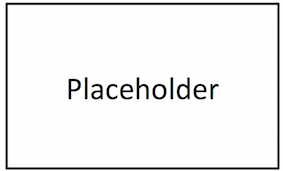
\includegraphics[width=0.9\columnwidth]{figures/placeholder.png}
Line graph, with vertical lines for cache sizes and a horizontal line for pin bandwidth.
Shows both ijk and ikj layout, demonstrates the TLB issue described in the tiling section.
For the ikj layout, demonstrates the five predictions we make in the tiling section.
1 Socket worth of cores, sweep minimum feasible tile size to something past L3 size.
\end{figure}

\begin{figure}%[thbp]
\centering
\caption{\textbf{Tile Size vs Bandwidth on Haswell:}}
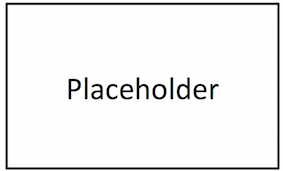
\includegraphics[width=0.9\columnwidth]{figures/placeholder.png}
Line graph, with vertical lines for cache sizes and a horizontal line for pin bandwidth.
Shows both ijk and ikj layout, demonstrates the TLB issue described in the tiling section.
For the ikj layout, demonstrates the five predictions we make in the tiling section.
1 Socket worth of cores, sweep minimum feasible tile size to something past L3 size.
\end{figure}

\begin{figure}%[thbp]
\centering
\caption{\textbf{Tile Size vs Bandwidth on Knight's Landing:}}
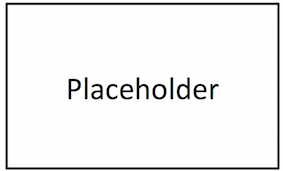
\includegraphics[width=0.9\columnwidth]{figures/placeholder.png}
Line graph, with vertical lines for cache sizes and a horizontal line for pin bandwidth.
Shows both ijk and ikj layout, demonstrates the TLB issue described in the tiling section.
For the ikj layout, demonstrates the five predictions we make in the tiling section.
1 Socket worth of cores, sweep minimum feasible tile size to something past L3 size.
\end{figure}

\begin{figure}%[thbp]
\centering
\caption{\textbf{Performance Impact of Optimizations on Ivy Bridge:}}
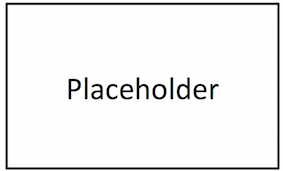
\includegraphics[width=0.9\columnwidth]{figures/placeholder.png}
Bar graph, left to right: MKL, NAMEFORALGO, pin bandwidth
For NAMEFORALGO, the stack (bottom to top) is: ijk repeated-div untiled no-mitigation, +mitigation, +tiling, +cached-div, +ikj
1 Socket worth of cores
\end{figure}

\begin{figure}%[thbp]
\centering
\caption{\textbf{Performance Impact of Optimizations on Haswell:}}
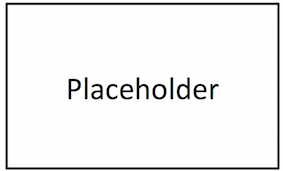
\includegraphics[width=0.9\columnwidth]{figures/placeholder.png}
Bar graph, left to right: MKL, NAMEFORALGO, pin bandwidth
For NAMEFORALGO, the stack (bottom to top) is: ijk repeated-div untiled no-mitigation, +mitigation, +tiling, +cached-div, +ikj
1 Socket worth of cores
\end{figure}

\begin{figure}%[thbp]
\centering
\caption{\textbf{Performance Impact of Optimizations on Knight's Landing:}}
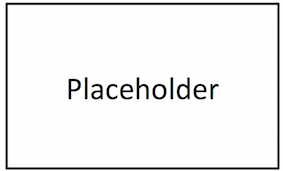
\includegraphics[width=0.9\columnwidth]{figures/placeholder.png}
Bar graph, left to right: MKL, NAMEFORALGO, pin bandwidth
For NAMEFORALGO, the stack (bottom to top) is: ijk repeated-div untiled no-mitigation, +mitigation, +tiling, +cached-div, +ikj
1 Socket worth of cores
\end{figure}

%\begin{table}%[htbp]
%\center
%\scriptsize
%\caption{\textbf{Comparison of Mixed-Precision and Double-Precision Algorithms}:
%To study the trade-off in performance and accuracy between the mixed-precision
%and double-precision variants of our algorithm, we solved a 1D diffusion
%problem with both codes on a single Intel Xeon ??? "Ivy Bridge" core. We used
%two measures to quantify error: the L2 norm of the difference between the
%analytic solution and the computing solution, and the absolute maximum of the
%residual vector of the tridiagonal solve. The test problem had storage
%requirements of approximately ~4.3 GB. 10 sample runs were performed with each
%sample performing 5 time steps. The walltime and uncertainty metrics below are
%normalized to the double-precision results; the L2 norm and residual metrics
%specify order of magnitude.
%}
%\small
%\setlength{\tabcolsep}{3pt}
%\begin{tabular}{|c|c|c|c|} \hline
%\textbf{Algorithm} & \textbf{Walltime (Normalized)} & \textbf{L2 Norm} & \textbf{Residual} \\ \hline
%Double-Precision   & 1.0   $\pm$ 0.007              & O(1e-07)         & O(1e-16)          \\ \hline 
%Mixed-Precision    & 0.836 $\pm$ 0.006              & O(1e-06)         & O(1e-08)          \\ \hline
%\end{tabular}
%\label{tab:mixed_vs_double}
%\end{table}

%\begin{figure}%[thbp]
%\centering
%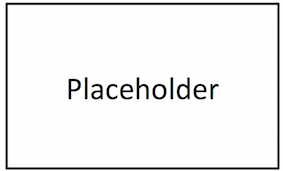
\includegraphics[width=0.9\columnwidth]{figures/placeholder.png}
%\caption{\fix{(Add the figure)} 
%Baseline performance using MKL (and hand) 
%using i-major data layout (not vectorized), for KNL, HSW.}
%\label{fig:tbd}
%\end{figure}

%\begin{figure}%[thbp]
%\centering
%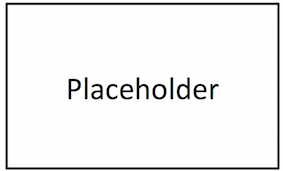
\includegraphics[width=0.9\columnwidth]{figures/placeholder.png}
%\caption{\fix{(Add the figure)} 
%Performance as a function of 32b RCP NR (not needed on KNL), stored
%reciprocal (cuts divides in half) for fixed file size (4?) }
%\end{figure}

%\begin{figure}%[thbp]
%\centering
%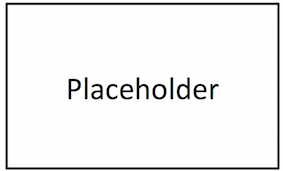
\includegraphics[width=0.9\columnwidth]{figures/placeholder.png}
%\caption{\fix{(Add the figure)} 
%Performance vs. Tile Size (jtile = 1,2,4,8,16,32) }
%\end{figure}

%\begin{figure}%[thbp]
%\centering
%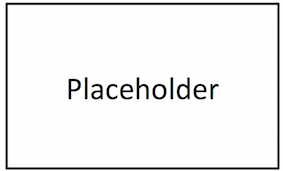
\includegraphics[width=0.9\columnwidth]{figures/placeholder.png}
%\caption{\fix{(Add the figure)} 
%Best Performance vs. MKL using same data layout vs. MKL using its best
%(include DRAM BW limit) }
%\end{figure}

%\begin{figure}%[thbp]
%\centering
%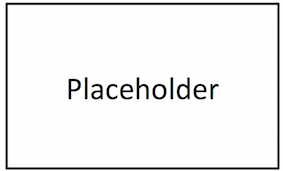
\includegraphics[width=0.9\columnwidth]{figures/placeholder.png}
%\caption{\fix{(Add the figure)} 
%Performance as a function of total parallelism for constant tile size
%[optional time permitting] }
%\end{figure}

%\begin{figure}%[thbp]
%\centering
%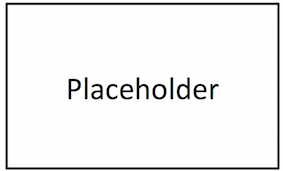
\includegraphics[width=0.9\columnwidth]{figures/placeholder.png}
%\caption{\fix{(Add the figure)} 
%Performance with 2,3,4 hyperthreads...  maybe just prose comments?  }
%\end{figure}

%\begin{figure}%[thbp]
%\centering
%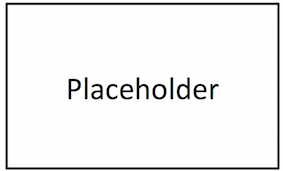
\includegraphics[width=0.9\columnwidth]{figures/placeholder.png}
%\caption{\fix{(Add the figure)} 
%effect of kdim != pow(2)... maybe just prose comments?  }
%\end{figure}

%\begin{figure}%[thbp]
%\centering
%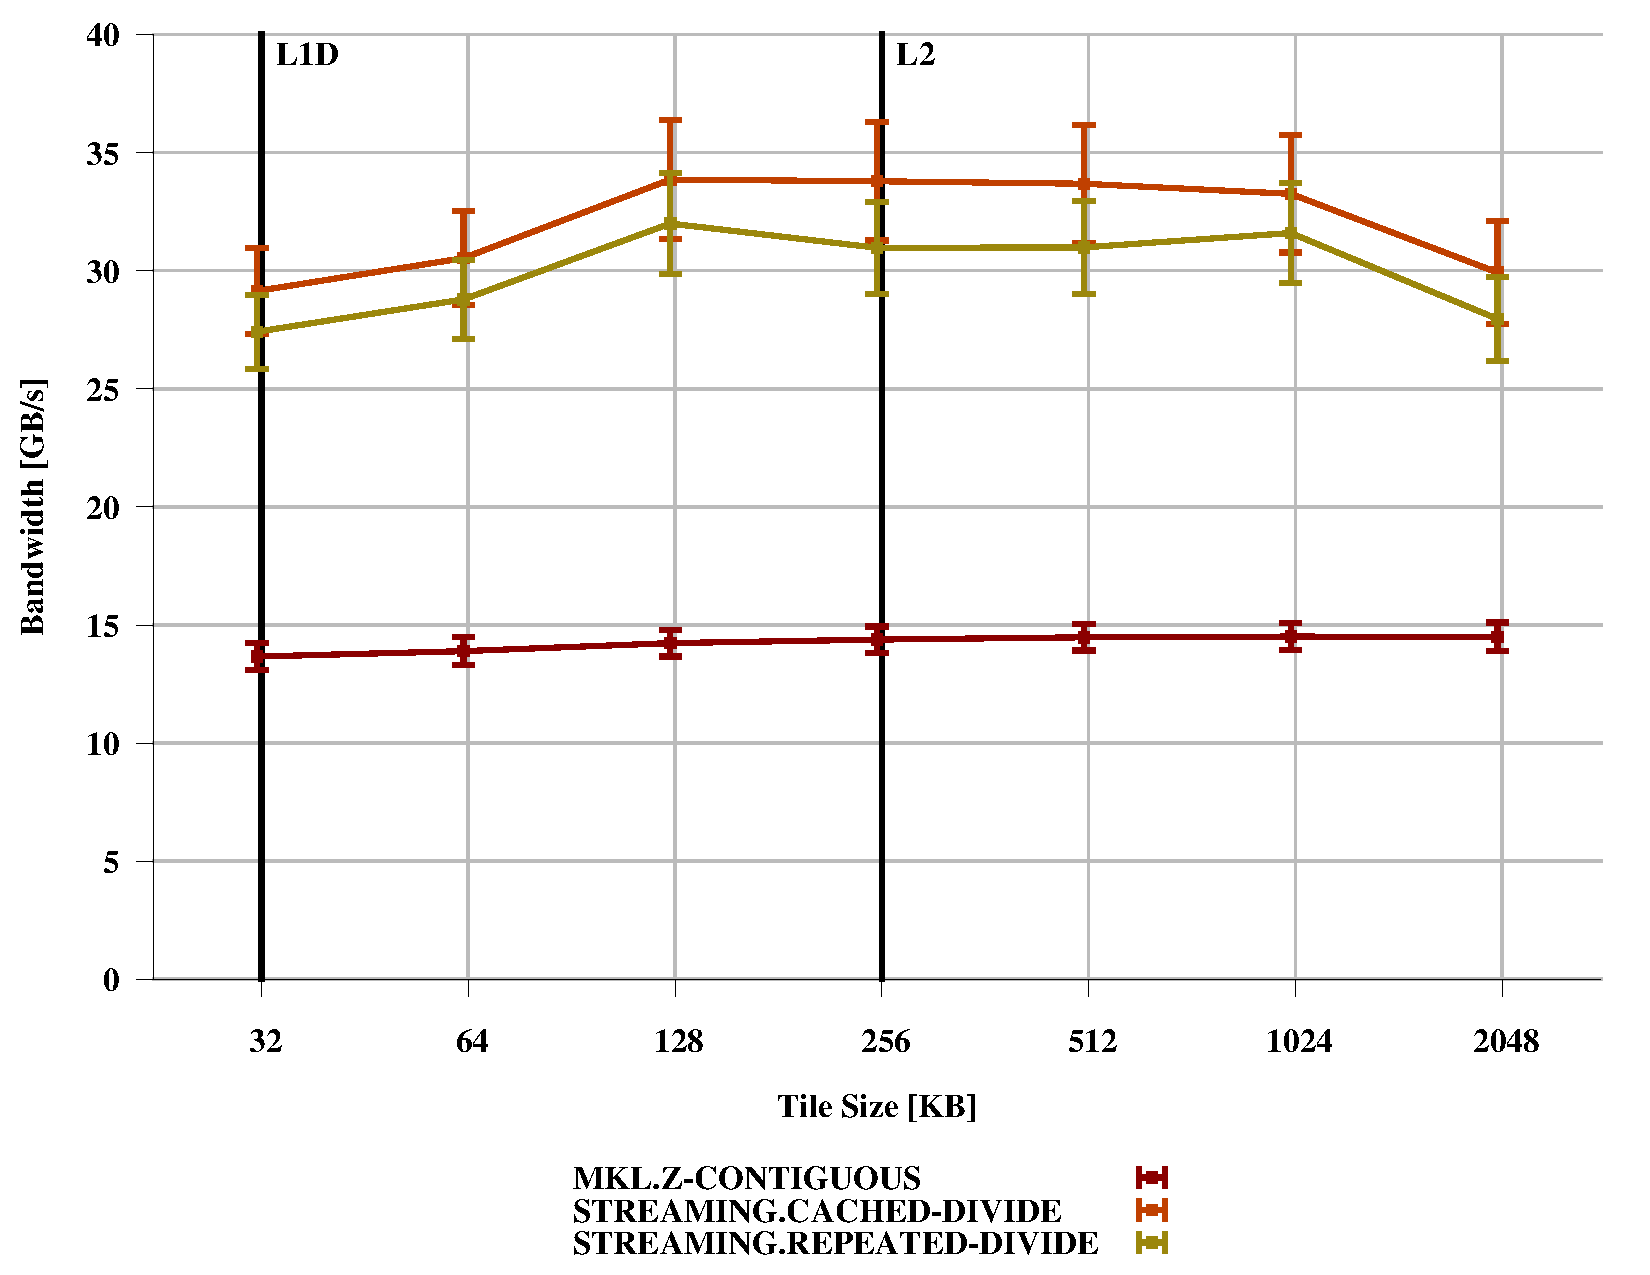
\includegraphics[width=0.9\columnwidth]{figures/post_tsb_tw_sweep_full_matrix_double_precision_production_snb_e5_2670_08_21_2016_8pus.pdf}
%\caption{\textbf{Tile Size vs Bandwidth on Sandybridge:}
%Measured bandwidth of the tridiagonal solve as a function of tile size on
%an Intel Xeon E5-2670 processor. The benchmark was run with 8 threads (each mapped
%to a single core of the CPU) and a 7.8 GB problem size. 190 sample runs were
%collected.}
%\end{figure}
%
%\begin{figure}%[thbp]
%\centering
%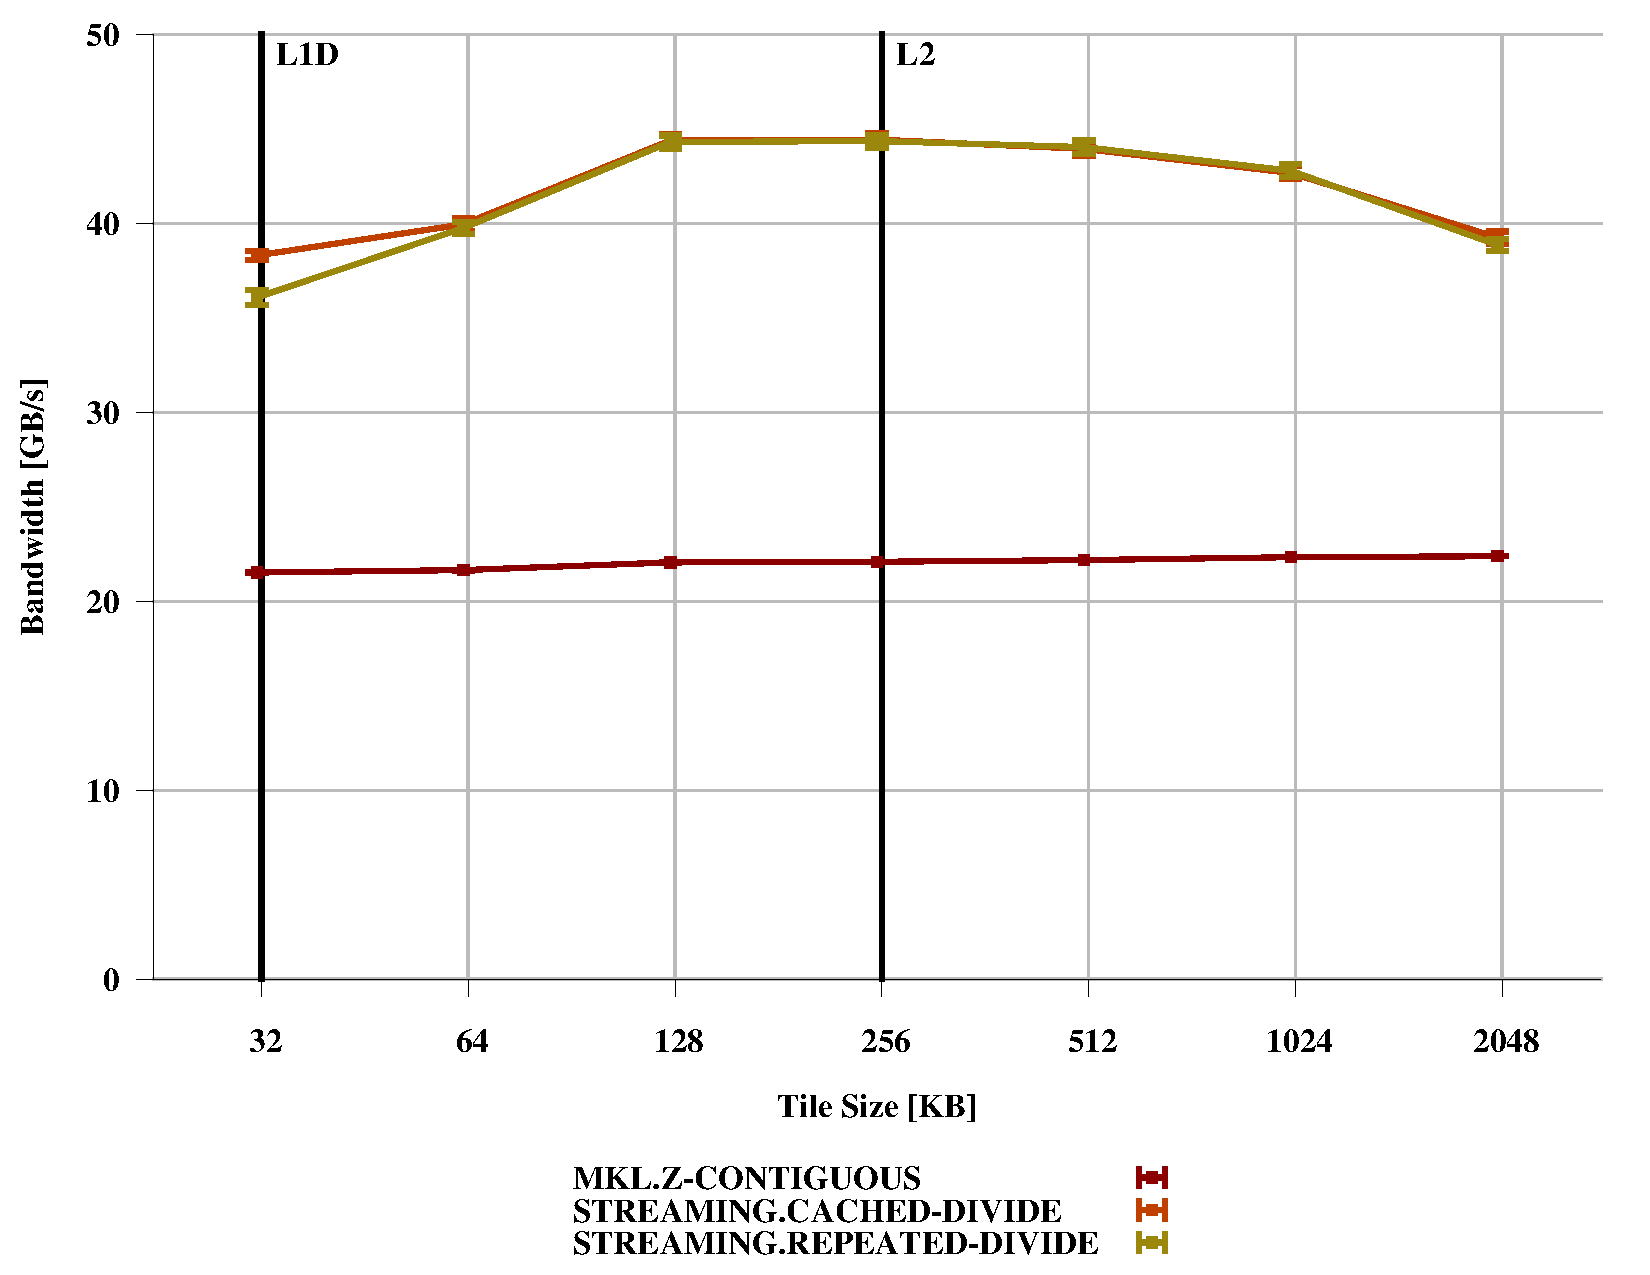
\includegraphics[width=0.9\columnwidth]{figures/post_tsb_tw_sweep_full_matrix_double_precision_production_ivb_e5_2695_v2_08_21_2016_12pus.pdf}
%\caption{\textbf{Tile Size vs Bandwidth on Ivybridge:}
%Measured bandwidth of the tridiagonal solve as a function of tile size on
%an Intel Xeon E5-2695 V2 processor. The benchmark was run with 12 threads (each
%mapped to a single core of the CPU) and a 7.8 GB problem size. 160 sample runs
%were collected.}
%\end{figure}
%
%\begin{figure}%[thbp]
%\centering
%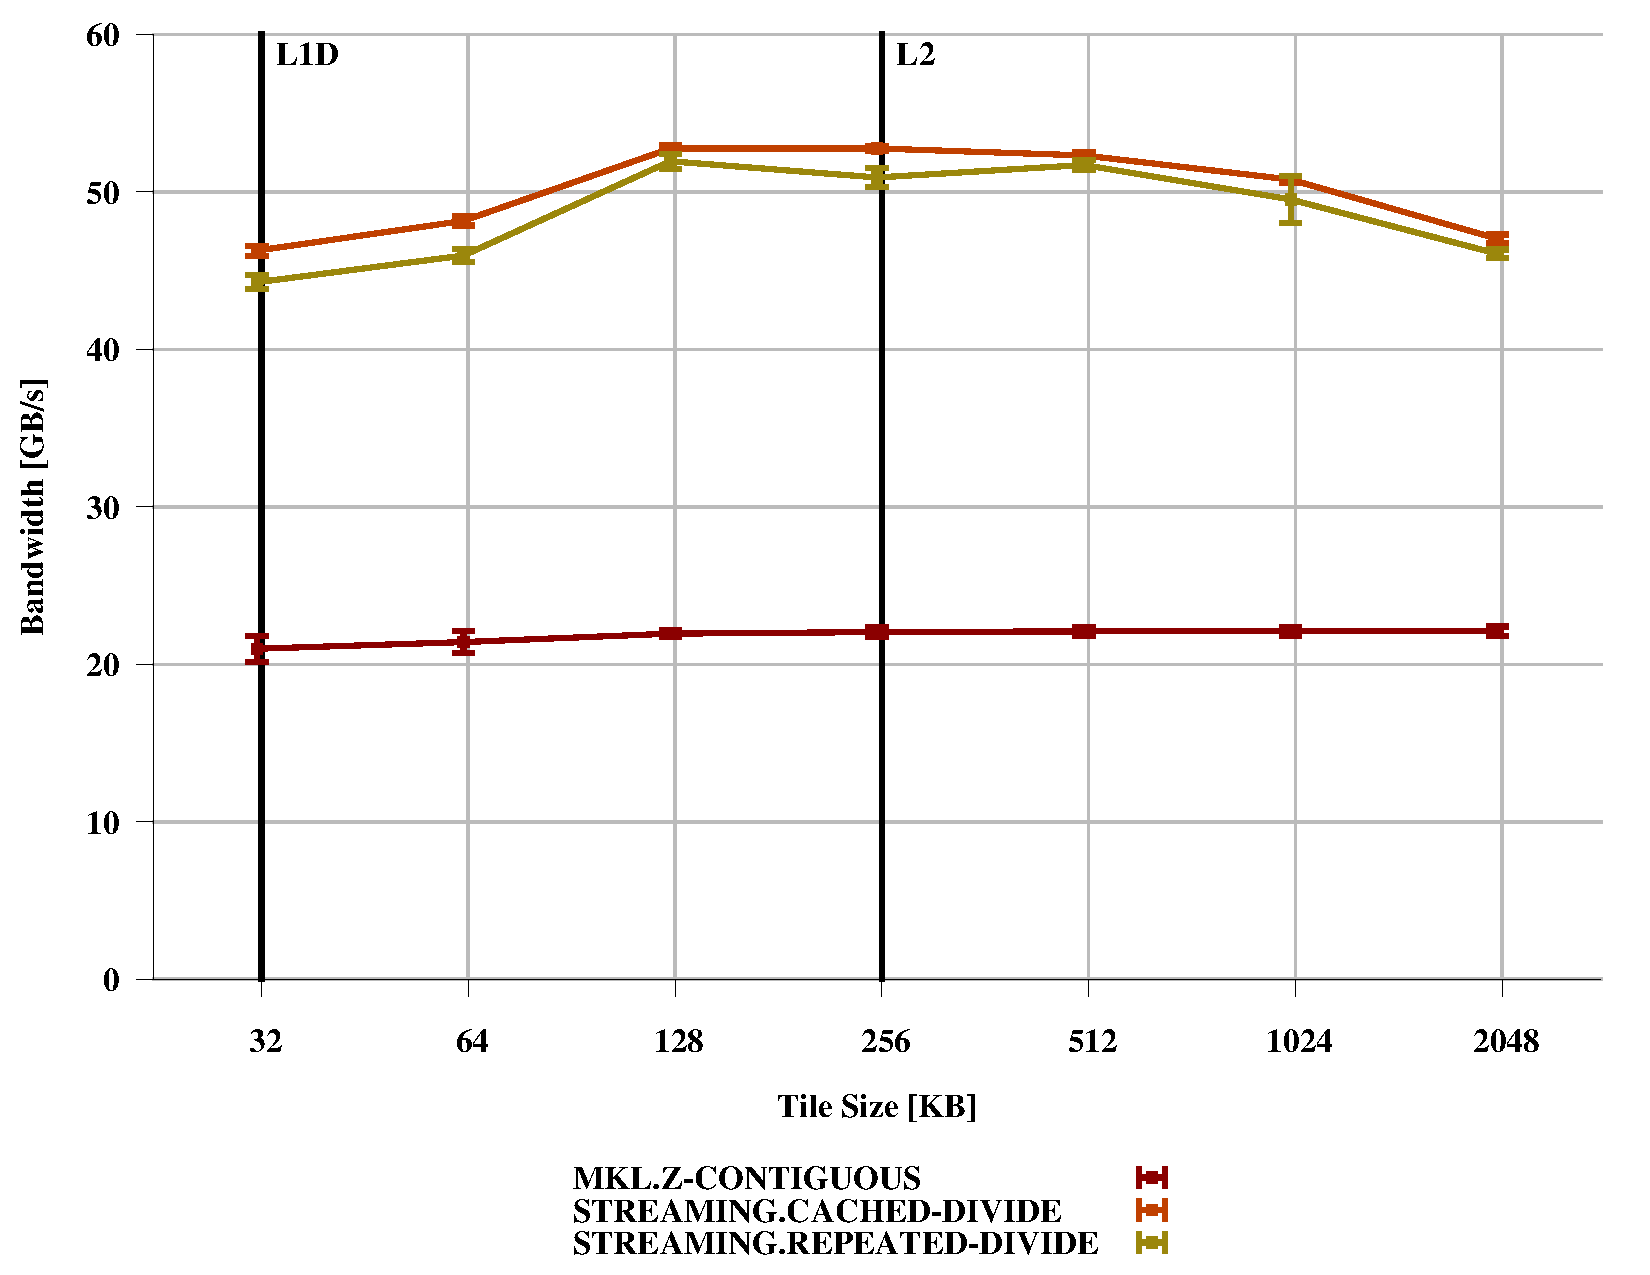
\includegraphics[width=0.9\columnwidth]{figures/post_tsb_tw_sweep_full_matrix_double_precision_production_hsw_e5_2670_v3_08_21_2016_12pus.pdf}
%\caption{\textbf{Tile Size vs Bandwidth on Haswell:}
%Measured bandwidth of the tridiagonal solve as a function of tile size on
%an Intel Xeon E5-2670 V3 processor. The benchmark was run with 12 threads (each
%mapped to a single core of the CPU) and a 7.8 GB problem size. 190 sample runs
%were collected.}
%\end{figure}
%
%\begin{figure}%[thbp]
%\centering
%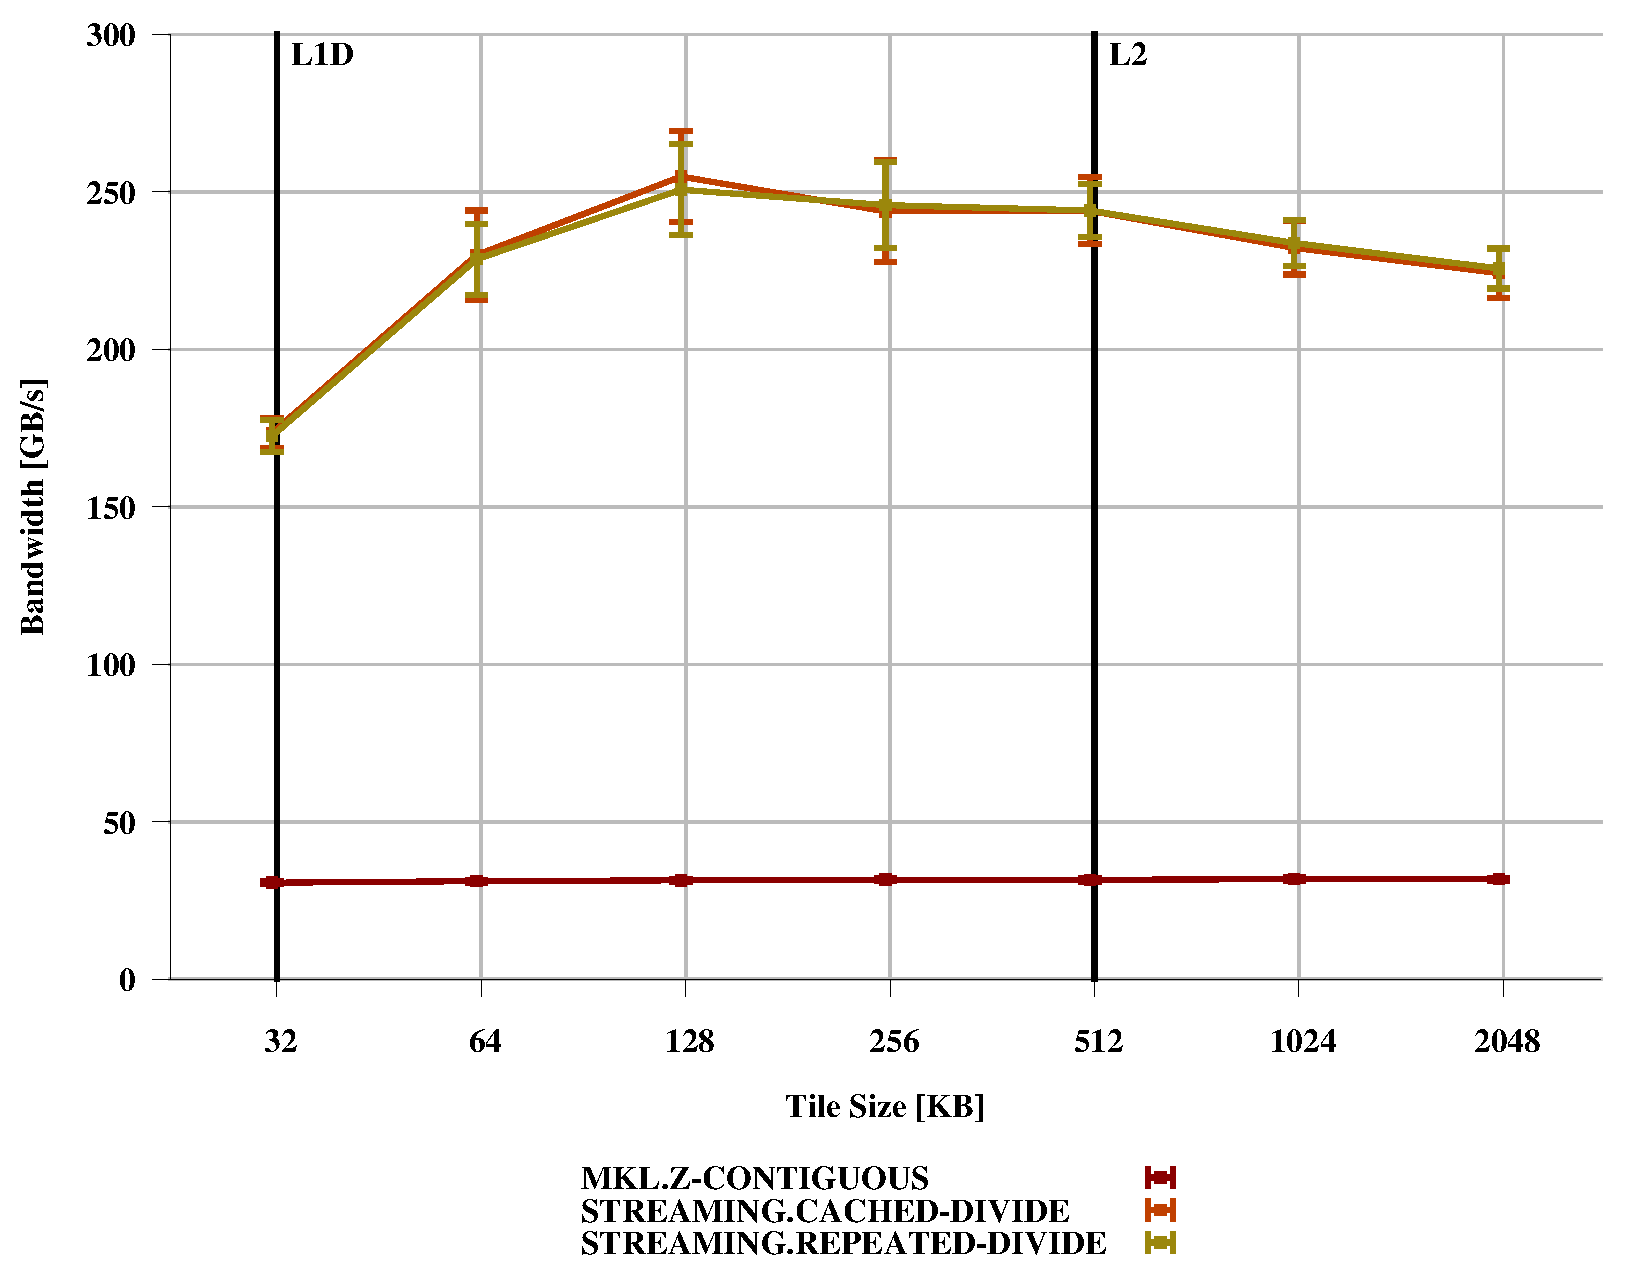
\includegraphics[width=0.9\columnwidth]{figures/post_tsb_tw_sweep_full_matrix_double_precision_production_knl_7210_08_21_2016_64pus.pdf}
%\caption{\textbf{Tile Size vs Bandwidth on Knight's Landing:}
%Measured bandwidth of the tridiagonal solve as a function of tile size on
%an Intel Xeon Phi 7210 processor. The benchmark was run with 64 threads (each
%mapped to a single core of the CPU) and a 3.9 GB problem size. 130 sample runs
%were collected. The processor was configured in the "quadcache" mode, where the
%16GB high-bandwidth memory is configured as a data cache.}
%\end{figure}

%===========================================================================
\section{Conclusion}

\section{Future Work}

\fxnote{Paragraph about rolling matrix}

\fxnote{Paragraph discussing combining the matrix build into the kernel}

% Need a section explaining tile size / tile storage size

% Future work should mention smaller tile sizes.

%===========================================================================
\section*{Acknowledgments}

\fxnote{Add Intel IPCC acknowledgments}

This material is based upon work supported by the U.S. Department of Energy, Office of Science, Advanced Scientific Computing Research, Scientific Discovery through Advanced Computing (SciDAC) program.
This research used resources in Lawrence Berkeley National Laboratory and the National Energy Research Scientific Computing Center, which are supported by the U.S. Department of Energy Office of Science's Advanced Scientific Computing Research program under contract number DE-AC02-05CH11231.  
This research used resources in Louisiana State University's Center for Computation and Technology. \fxnote{Check with Adrian if there's wording here that LSU likes}

%This research used resources of the National Energy Research Scientific Computing Center (NERSC), which is supported by the Office of Science of the U.S. Department of Energy under contract DE-AC02-05CH11231.
%This research used resources of the Argonne Leadership Computing Facility at Argonne National Laboratory, which is supported by the Office of Science of the U.S. Department of Energy under contract DE-AC02-06CH11357.
%This research used resources of the Oak Ridge Leadership Facility at the Oak Ridge National Laboratory, which is supported by the Office of Science of the U.S. Department of Energy under Contract No. DE-AC05-00OR22725.


%===========================================================================
\bibliographystyle{IEEEtran}
\bibliography{sc16-implicit}
%===========================================================================

%===========================================================================
% 

%\section*{Notes/Outline}
%Submission info:
%\url{https://easychair.org/conferences/?conf=pmbs16}
%
%\begin{itemize}
%\item Climate apps use HE-VI model 3D+1D. Also a pattern for 2D+1D and 3D+0D chemistry
%\item Results demonstrate importance of ``batching'' solves, MLK doesn't do
%\item Cache coherency is important: IMEX RK accum, tiling
%\item Explicit part is HO stencil op, memory b/w bound (w/ ghost cells)
%\item Implicit part is non-linear solver: App requires different matrix at each i,j index 
%\item Results in repeated vertical sparse banded solve
%\item Solve (tridiag, banded, dense) should vectorize on i (unit stride), tiled in pencils
%\item Considerations for vector alignment, tiling, and memory
%\item Performance results, scaling, comparison, by platform / parameter
%\item Future work: communication hiding, load imbalance, IMEX
%\end{itemize}
%(Bryce's email comments) Looking over the outline:
%\\
%It's crucial that we clearly identify the optimizations that we
%believe are novel/high-impact, vs the optimizations that are
%well-known to the community (even if they were not well known to us).
%For example, on the outline, we have listed "IMEX RK accum, tiling".
%Do we want to present the accumulation optimizations which removed
%unnecessary temporaries from the time integrator? Do we feel that
%optimization is novel, or is that just a common-sense thing that only
%affected us because of the Chombo programming model? Likewise, do we
%want to present tiling as a focal point in this paper? Tiling is a
%well-known technique; we certainly can't claim tiling in general as
%novel work. Is some part of our tiling approach novel? (how about
%parallelizing the tile loop - is that fairly novel? I know Sam does
%this in HPGMG, but is this a widely used technique?)
%\\
%We would be well served by applying the scientific method at this juncture:
%\\
%\begin{itemize}
%\item Question: What concrete research question(s) are we answering?
%\begin{itemize}
%\item Prior research indicates that HE-VI methods show promise as a
%scalable approach to solving global climate problems on cubed sphere
%geometries because <explanation> [cite prior studies]. How do we
%implement HE-VI methods which perform well on cache-coherent SIMD
%architectures?
%\item When solving a problem with a high horizontal-vertical aspect ratio
%(e.g. the horizontal extents are much greater than the vertical
%extents) with HE-VI methods, it is necessary to perform a large number
%of small vertical implicit solves (<give examples of matrix sizes>
%[citation]) which are independent of each other. <explain the type of
%solves in the climate dycore - e.g. non-linear but nearly banded>
%[citation]. How can we efficiently solve large quantities of small
%non-linear bandedish/banded/tridiagonal matrices on cache-coherent
%SIMD architectures?
%\end{itemize}
%\item Hypothesis: What theories did we come up with that would answer our
%research question(s)?
%\begin{itemize}
%\item Optimal memory access patterns, management of working set sizes
%(e.g. staying in cache) and efficient use of vector units are
%necessary to achieve good performance on cache-coherent SIMD
%architectures.
%\begin{itemize}
%\item Optimal memory access patterns: moving through memory in unit
%stride, controlling the number of streams.
%\item Management of working set sizes: tiling, reducing size of
%temporaries/localizing temporaries (thread-local or otherwise)
%\item Efficient use of vector units: moving through memory in unit
%stride, controlling memory alignment, controlling array strides,
%annotation-assisted autovectorization
%\item TODO: List of individual, concrete optimizations from above.
%\end{itemize}
%\item Mainstream linear algebra libraries (<examples> [citation]) are not
%well-suited for solving large quantities of small non-linear
%bandedish/banded/tridiagonal matrices on cache-coherent SIMD
%architectures because <expalanation> [cite prior studies if possible].
%\end{itemize}
%
%
%\item Prediction: If our hypotheses are true, what results can we expect to
%see? \\
%$\rightarrow$ TODO: What performance characteristics should we see with and
%without each of the concrete optimizations from our hypothesis above?
%
%\item Experiment: Investigate the predictions we've made. \\
%$\rightarrow$ TODO: Methodology for benchmarking the optimizations identified
%above and measuring the performance characteristics we're interested
%in.
%
%\item Analysis: What were the results of our experiments?
%\end{itemize}
%
%List of figures from meeting on 8/11:
%For KNL, HSW, SNB(?)...
%List of figures from meeting on 8/11:
%-For KNL, HSW, SNB(?)...
%\begin{enumerate}
%\item Baseline performance using MKL (and hand) using i-major data layout 
%(not vectorized)
%\item Performance as a function of 32b RCP NR (not needed on KNL), stored
%reciprocal (cuts divides in half) for fixed file size (4?)
%\item Performance vs. Tile Size (jtile = 1,2,4,8,16,32)
%\item Best Performance vs. MKL using same data layout vs. MKL using its best
%(include DRAM BW limit)
%\item Performance as a function of total parallelism for constant tile size
%[optional time permitting]
%\item Performance with 2,3,4 hyperthreads...  maybe just prose comments?
%\item effect of kdim != pow(2)... maybe just prose comments?
%\end{enumerate}


\end{document}


